\begin{frame}
    \frametitle{Automatizované testování}

    \begin{block}{Automatizované testování}
        Automatizací testů si ušetříme práci a zároveň získáme jistotu, že naše knihovna funguje tak, jak má.
        Programy pro automatizované testování nám také mohou poskytnout informaci o pokrytí kódu testy.
    \end{block}

\end{frame}

\begin{frame}
    \frametitle{Automatizované testování - Jest}
    \framesubtitle{Spouštěné lokálně v příkazové řádce}
    \begin{figure}
        \centering
        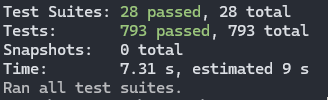
\includegraphics[width=0.8\textwidth]{../resources/tests.png}
        \caption{Výsledek automatizovaných testů pomocí Jestu.}
    \end{figure}
\end{frame}

\begin{frame}
    \frametitle{Automatizované testování - Jest}
    \framesubtitle{Automaticky spouštěné při pushi na GitHub}
    \begin{figure}
        \centering
        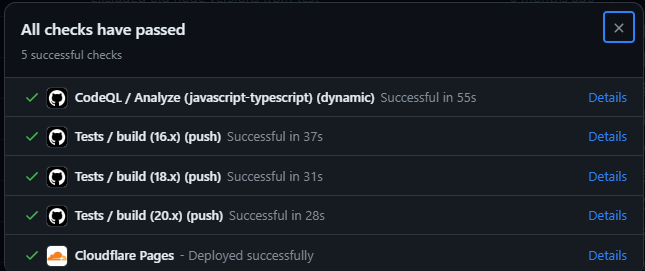
\includegraphics[width=0.8\textwidth]{../resources/tests-github.png}
        \caption{Výsledek \uv{GitHub Actions} při pushi na GitHub.}
    \end{figure}

\end{frame}

\begin{frame}
    \frametitle{Automatizované testování - Jest}
    \framesubtitle{Automaticky spouštěné při pushi na GitHub}
    \begin{figure}
        \centering
        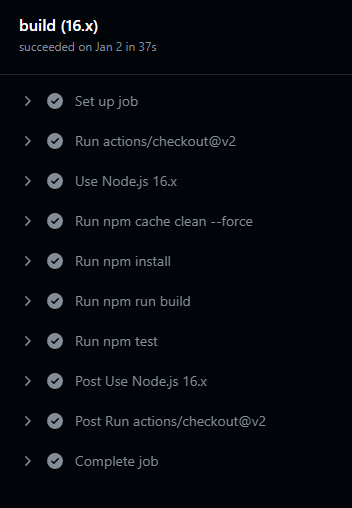
\includegraphics[height=0.6\textheight]{../resources/tests-github-16.png}
        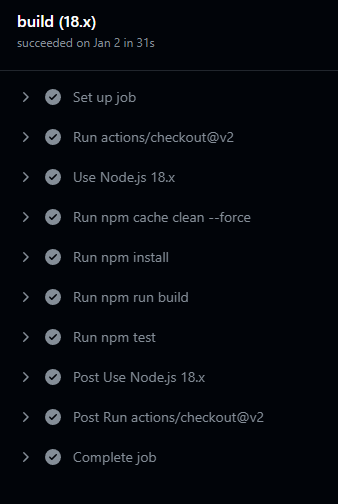
\includegraphics[height=0.6\textheight]{../resources/tests-github-18.png}
        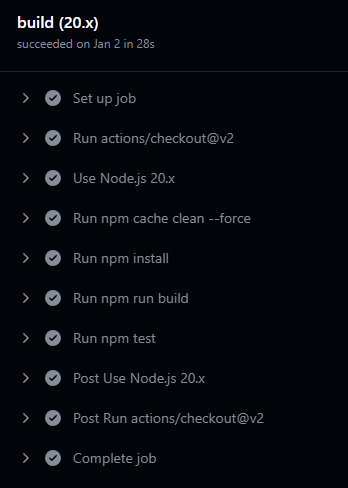
\includegraphics[height=0.6\textheight]{../resources/tests-github-20.png}
        \caption{Podrobný výsledek testů při pushi na GitHub.}
    \end{figure}

\end{frame}
